This chapter creates an understanding of the given data, how it is analysed and prepared before including it in deep learning models. Thereto the different programs respectively the program where pain maps are created and the program for development of the deep learning models. **** ADD SOMETHING ABOUT DEEP LEARNING (MADS AND IGNAS) ****


\section{Data}
Data used in this project were collected beforehand from an on-going FOXH trial which is conducted in collaboration with Danish and Australian universities. The data consists of pain maps which were drawn by individuals with PFPS through the use of an application, Navigate Pain, in a clinical setting. Navigate pain is further described in section \ref{sec:nav}. The pain maps both from individuals with uni- and bilateral PFP. An example of a pain drawing with bilateral pain is shown in figure \ref{fig:kneepainmap}.

\begin{figure} [H]
\centering
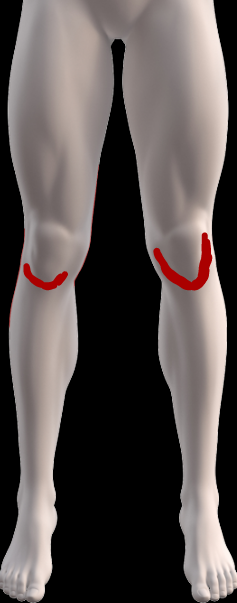
\includegraphics[width=0.27\textwidth]{figures/kneepainmap}
\caption{Pain drawings of the lower extremities. The red markings indicate the area of pain perceived by the individuals. In this case the PFP is bilateral (on both knees).}
\label{fig:kneepainmap}
\end{figure}

\noindent
In addition to the pain maps an appurtenant dataset was available. This contained information regarding the individuals in terms of i.a. age, gender, symptom duration, pain intensity and the most prominent knee for pain.
Before using the data in the deep learning models, a manual data handling was necessary. This incorporate matching the given pain maps and appertaining ID regarding the individuals, which resulted in 217 pain maps. Furthermore specific information like gender, symptom duration and pain intensity are collected. The number of pain maps and associated information, gender and symptom duration, is 205. Additionally, there were 197 pain maps with associated information, gender and pain intensity.


\subsection{Software application: Navigate Pain} \label{sec:nav}
Navigate Pain is a software application that is used to visualise the location, shape and spatial distribution of pain from patient to healthcare personnel. The application permits individuals to draw their pain into a body outline with different colors and line thickness. Navigate Pain android was developed at Aalborg University and a commercial web application is available at Aglance Solutions (Denmark).\citep{Solutions2015}
\autoref{fig:Navigatepain} illustrates the process using the application.

\begin{figure} [H]
\centering
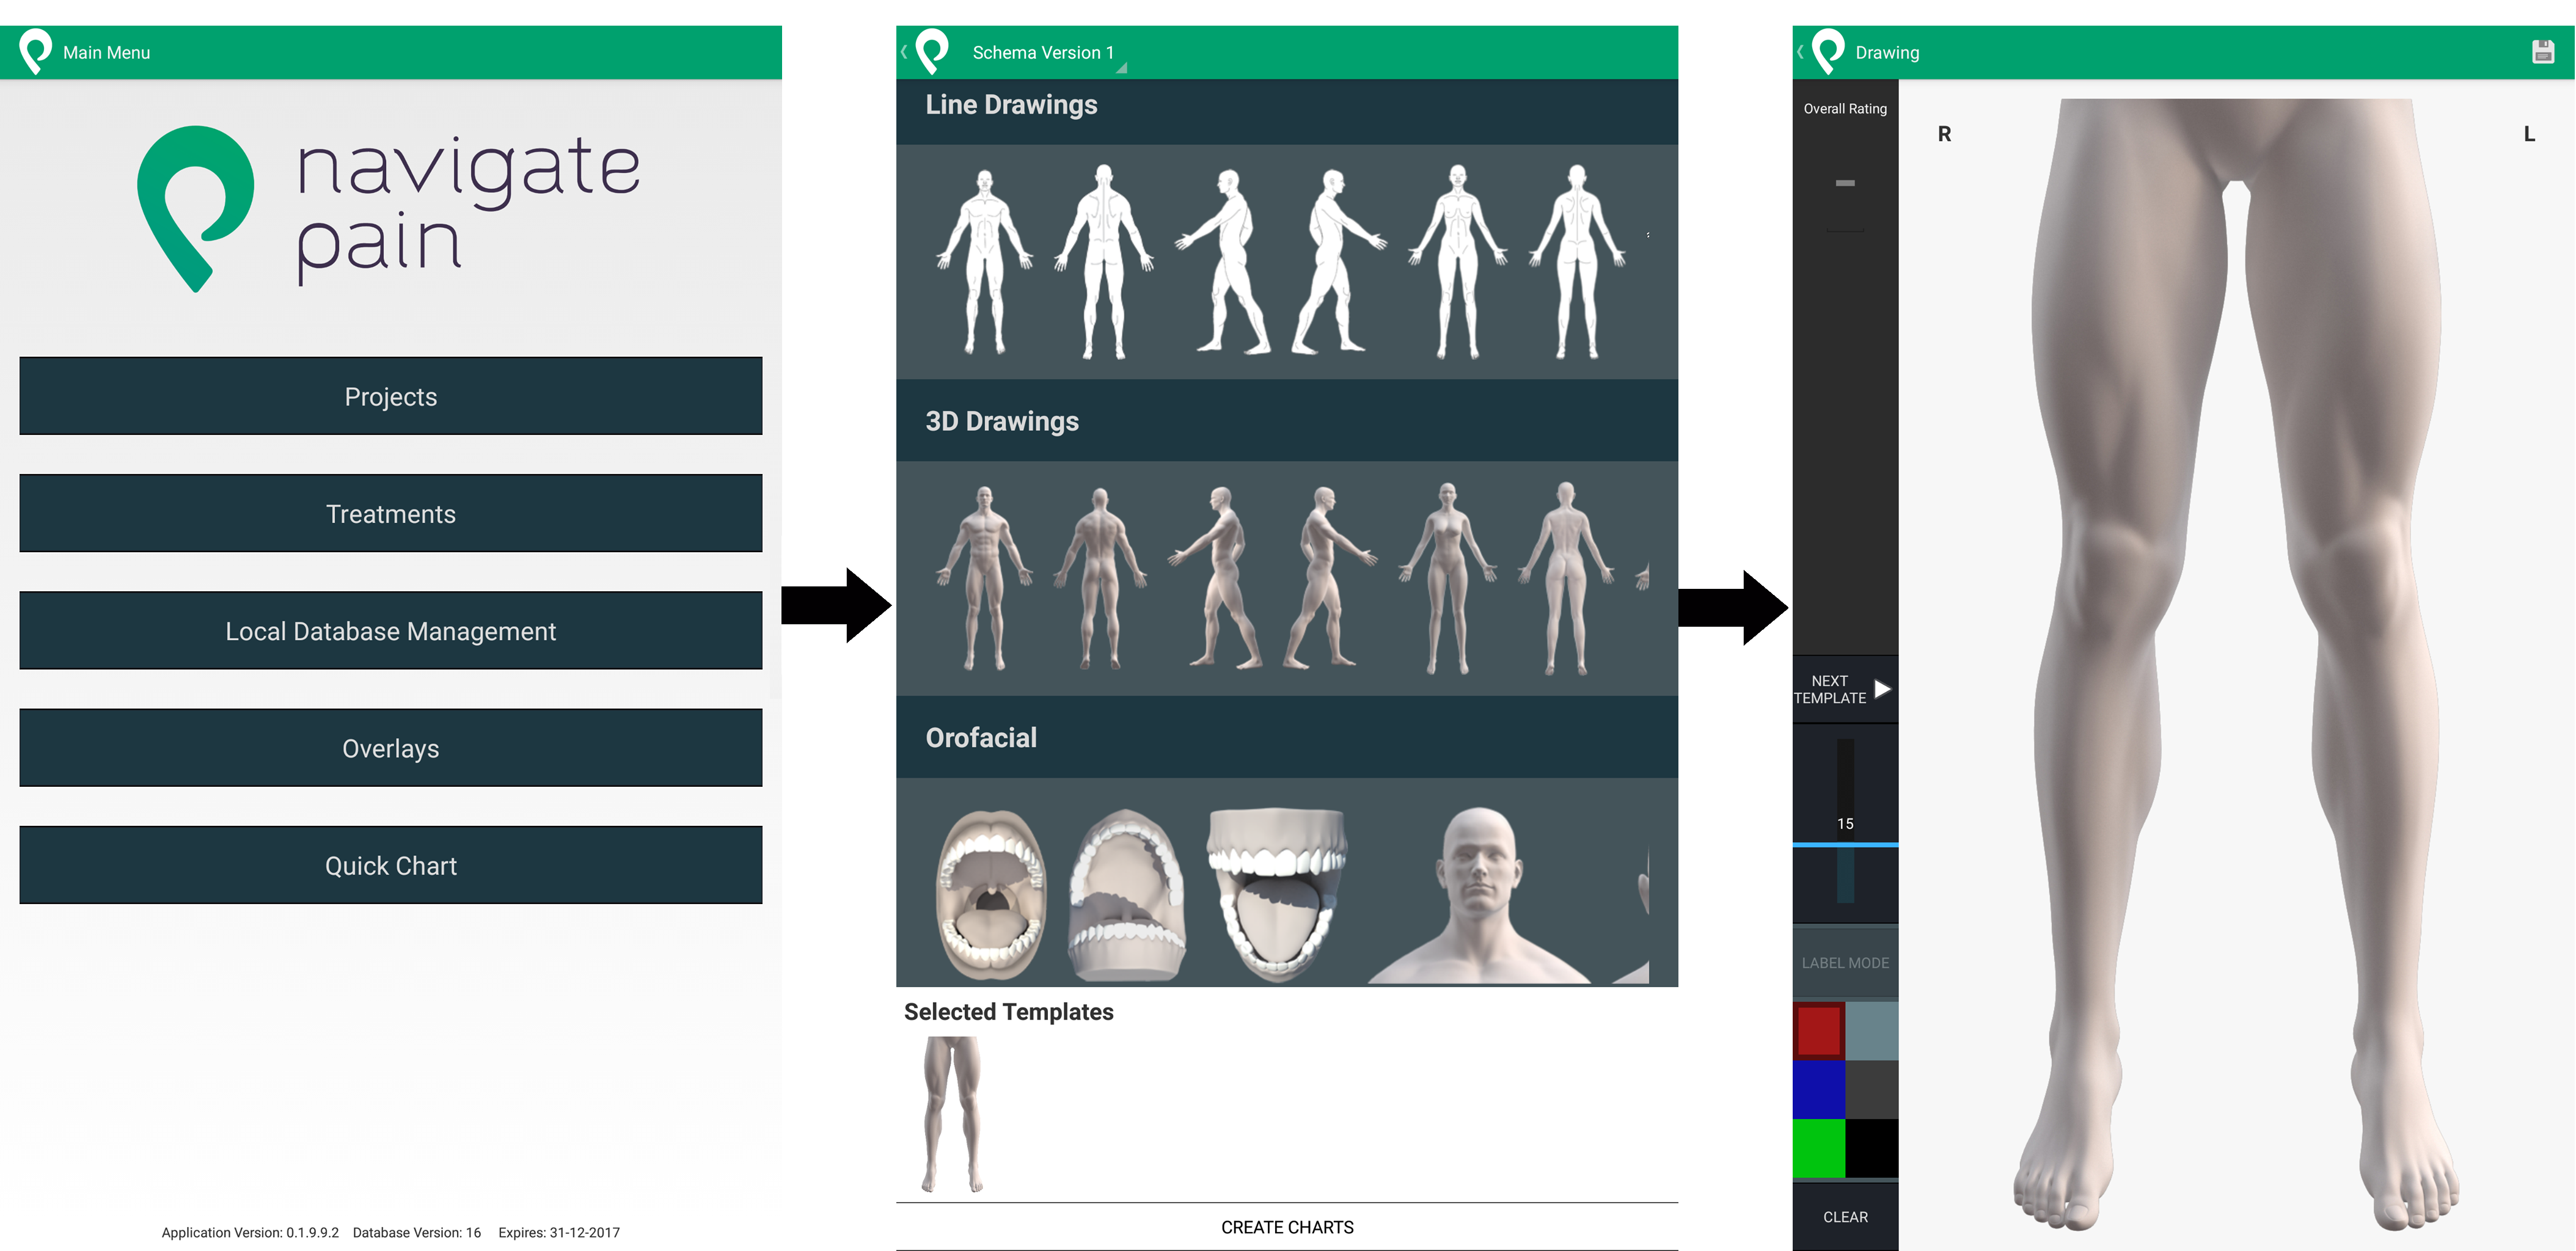
\includegraphics[width=1\textwidth]{figures/Navigatepain}
\caption{The process for making a pain map with Navigate Pain. (a) shows the main screen, (b) categories of body outlines and (c) body outline for lower extremities.}
\label{fig:Navigatepain}
\end{figure}

\noindent
The left screen in figure \ref{fig:Navigatepain}(a) is the main screen. By clicking on "Project", a folder with individuals is created. From each individual information like name, age, height is saved. Before the individual can draw their pain areas, the body outline has to be chosen, which is illustrated in figure (b). The body outlines are divided into five categories: Line Drawings, 3D Drawings, Orofacial, Special Zooms and Knee Pain. In the bottom the seleceted templates are shown. When clicking on "CREATE CHARTS" the screen in figure (c) is shown. Here it is possible to draw the pain areas with different colors and line thickness, which can be seen in the left side of the screen. Afterwards the pain map can be saved.


\subsection{Data representations} \label{sec:representation}
It is presumed that different representations of the pain maps affect the performance accuracy of a deep learning models, which is why different data representations are created.
A study by \citeauthor{Boudreau2017} found a correlation between a prolonged symptom duration and the size of the pain area. It was shown that the pain area increased for individuals that have a symptom duration for longer than five years compared to those with a symptom duration below. Likewise, pain intensity had a correlation with the size of pain area for individuals with a symptom duration for more than five years. Furthermore, the shape of the pain developed from a U-shape to an O-shape for individuals with a symptom duration above five years.\citep{Boudreau2017} \\
Based on this study the morphology of PFP is considered to be relevant to investigate, which is why morphology is the first data representation.\\

\noindent
The PFP is often described as diffuse pain and it is therefore difficult to describe and localise \citep{Witvrouw2014}. To accommodate this is it chosen to divide the pain into different knee regions, which may indicate whether a specific region of the knee influence the PFP. This is converted to a simplified data representation that indicate active knee regions.
A combination of the two data representations is created to achieve a third data representation which both include the morphology of the pain and the different active knee regions.
\noindent
Furthermore is gender an interesting parameter to use as an input, because the prevalence is more than twice as high for females than males. Thereto perceived pain is subjective and depends on the individual's character and personality. The distribution of gender is investigated by creating a histogram, which is shown in figure \ref{fig:histogender}.

\begin{figure} [H]
\centering
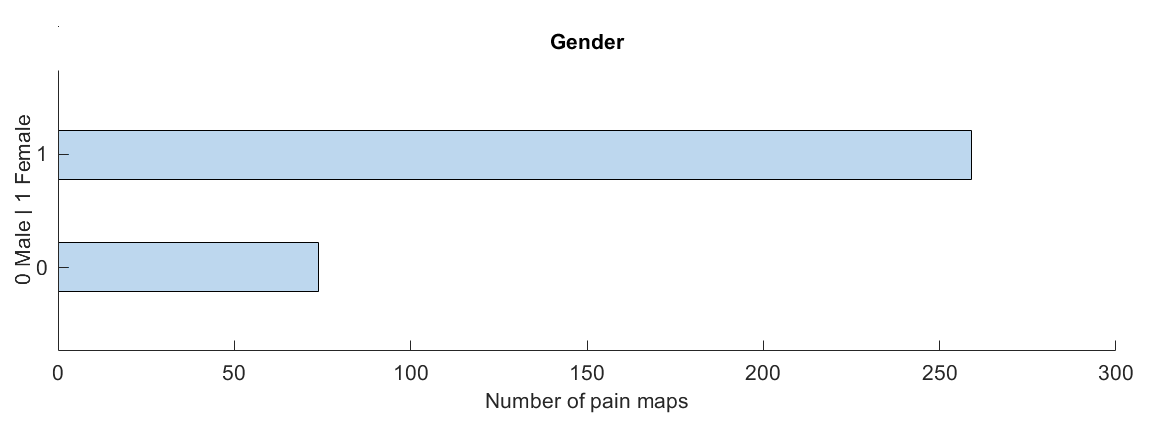
\includegraphics[width=1\textwidth]{figures/histoGender}
\caption{Histograms of the distribution of gender.}
\label{fig:histogender}
\end{figure}

\noindent
According to the given data the prevalence is higher for females than males. The females constitute 156 of the 206 individuals.


\noindent
Since the symptom duration of PFP seems to affect the size and shape of the pain area, is it chosen to classify the three data representations in proportion to symptom duration. Likewise is it chosen to classify pain intensity because of the influence from the size of pain area. Thereto is it interesting to investigate whether there is a connection between knee regions and either symptom duration or pain intensity.
The three data representations is referred to as morphology-, regions- and combined-representation.
\newpage

\section{Pre-analysis}
The pain maps and associated symptom duration as well as pain intensity are analysed to get an overview of the data. The data is analysed in MatLab, where the distribution of the outputs, symptom duration and pain intensity, are investigated whereafter classification to the deep learning models are decided. Furthermore are different threshold values analysed according to five pain maps to select the threshold which should define when a region is active. Lastly, a reference to the deep learning models is created to investigate whether the size of pain areas can predict either symptom duration or pain intensity by using a simple linear regression.


\subsection{Classification of data}
The deep learning models should classify the input, pain maps and gender, in different categories in relation to symptom duration or pain intensity intervals. To find these intervals are histograms of the both symptom duration and pain intensity created.

\noindent
A histogram of the symptom duration associated with the pain maps is illustrated in figure \ref{fig:histoduration}.

\begin{figure} [H]
\centering
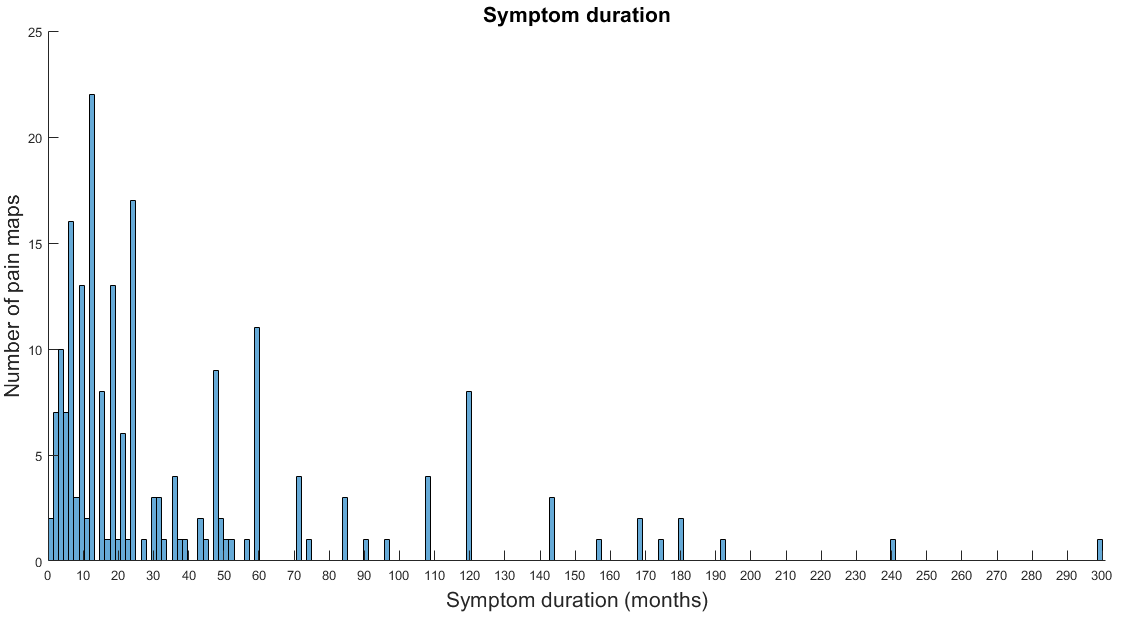
\includegraphics[width=1\textwidth]{figures/histogramDuration}
\caption{A histogram of the symptom duration.}
\label{fig:histoduration}
\end{figure}

\noindent
The symptom duration is divided into some classes which the models should classify in addition to. To test the models are the data firstly divided into two extremes, since it is assumed that if the models predict badly with the extremes, the models will not predict better with multiple classifications of symptom duration. The histogram is evaluated and thereby are the extremes chosen to be 0 to 12 and 36 to 300 months. Afterwards is the interval between used as a third classification. 
\noindent
In the appurtenant data to the pain map the individuals have stated their pain intensity as the worst pain in the last 24 hours and the last seven days.
It is not assumably that the individuals have performed any PFP provoked activity in the last 24 hours before drawing their pain, therefore it is chosen to use the worst pain intensity in the last seven days to get a more average value for the worst pain intensity.
To explore the difference between the individuals’ stated pain intensity in the last seven days is a histogram created which can be seen in figure \ref{fig:histopain}.

\begin{figure} [H]
\centering
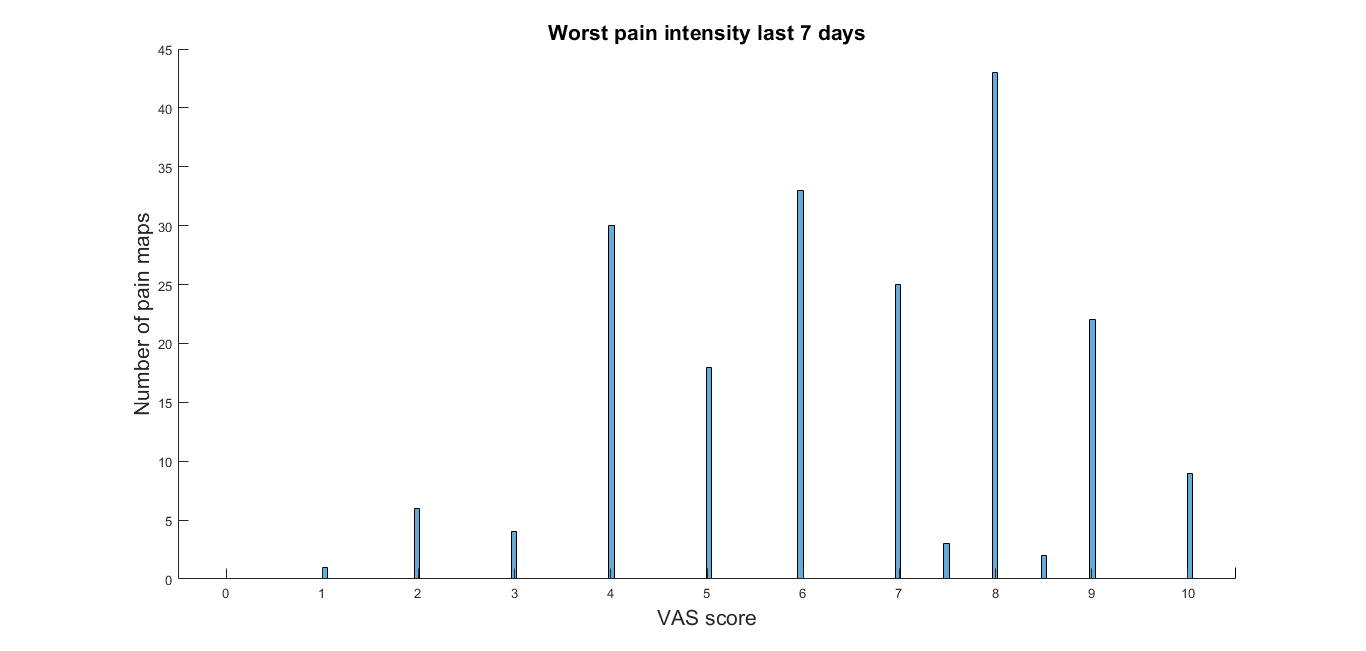
\includegraphics[width=1\textwidth]{figures/histrogramPain}
\caption{Histograms of the pain intensity the last seven days.}
\label{fig:histopain}
\end{figure}

\noindent
Likewise to the symptom duration classification, is the worst pain intensity divided into some into the extremes, which are chosen to be intervals 1 to 4 and 8 to 10. The third classification constitute the interval between the extremes.


\subsection{Threshold selection}\label{sec:Selectthreshold}
In relation to the data representation that contains information about the active pain regions, it is necessary to find a threshold that decides when a knee region contains enough pain pixels to be considered active. A threshold is required to increase the confidence of an active pain region by avoiding minimal contributions e.g. small pain areas in the associated regions. Simultaneously the threshold may not be too large so that potential pain regions will not be incorporated. The threshold to indicate active pain regions is decided based on an analysis, where threshold values of 0, 5, 10 and 15 percent are tested. The analysis of the threshold is tested on five random pain maps to get a general impression of the data. To better illustrate the division of the pain regions are the regions in figure \ref{fig:atlas} colored in different colors that are easier to distinguish, which is shown in figure \ref{fig:colorregion}.

\begin{figure} [H]
\centering
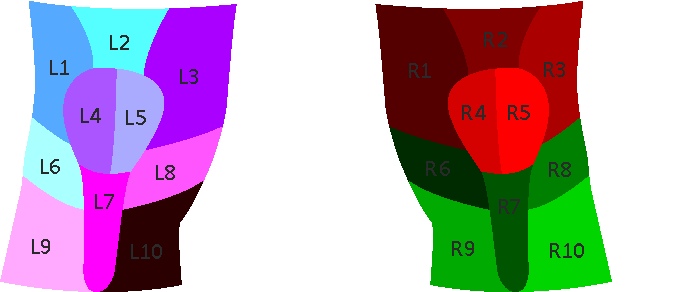
\includegraphics[width=0.6\textwidth]{figures/colorregion}
\caption{Knee regions colored in colors that are easier to distinguish.}
\label{fig:colorregion}
\end{figure}

\noindent
An example of pain maps and appurtenant bar chart are illustrated in figure \ref{fig:threshold}. The pain maps, figure \ref{fig:threshold}(a-d), are likewise colored in the same colors as figure \ref{fig:colorregion} to indicate which regions that are affected according to 0, 5, 10 and 15 percent threshold. The last figure (e) is the bar chart that indicates how many and which active regions there are according to the threshold values.

\begin{figure} [H]
\centering
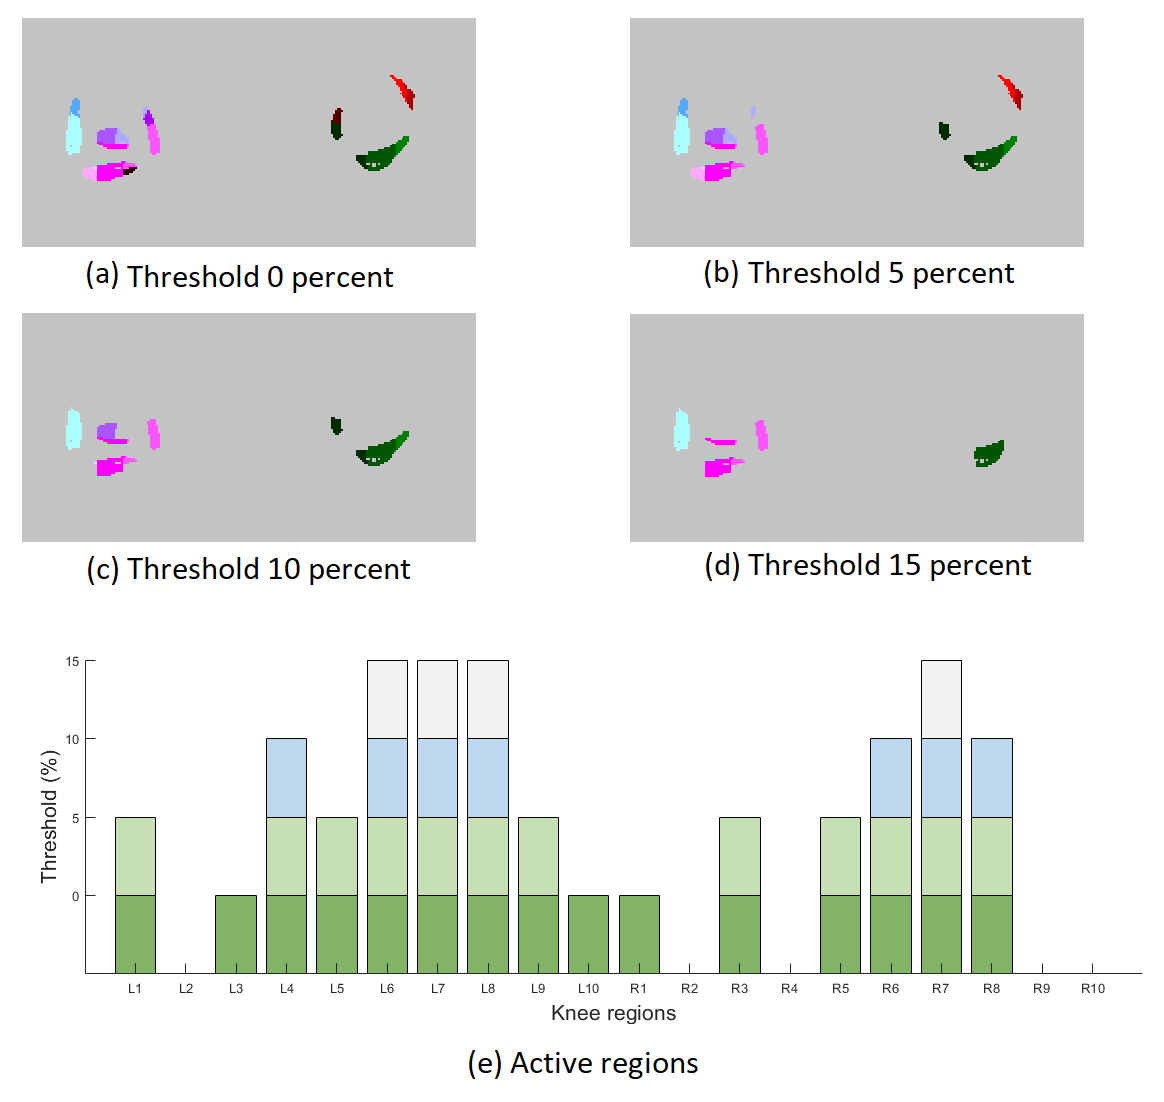
\includegraphics[width=0.95\textwidth]{figures/threshold4}
\caption{The active knee regions when the threshold is (a) 0 percent, (b) 5 percent, (c) 10 percent and (d) 15 percent. (e) is the bar chart that indicates how many and which knee regions that are considered active.}
\label{fig:threshold}
\end{figure}

\noindent
According to figure \ref{fig:threshold} (a) and (e) is it shown that the knee to the left has nine active regions and the knee to the right has six active knee regions, when the threshold is zero. In proportion to the active regions are region L3, L10 and R1 very small and are thereby the first regions to be discarded when the threshold is increased by 5 percent, which is shown in figure (b).
By comparing figure (a) and (b) can minor changes according to the missing regions be seen, compared to figure (c) and (d) where greater areas disappears after increasing the threshold to 10 and 15 percent.
\noindent
Based on analysis of the five pain maps and bar charts, figure \ref{fig:threshold} and appendix \ref{app:thresholds}, is a threshold on 5 percent chosen to avoid including minor pain areas, like region L10, as active knee regions, and to avoid discarding too many and large areas, like regions R3 and R5.


\subsection{Simple regression models}
To explore whether there is a simple correlation between a single feature and either symptom duration or pain intensity, are plots created. In relation to the data representations, morphology and regions, is it chosen to investigate two single features in relation to the representations. The features are number of pain pixel and active pain regions. The two features are visualised according to each output, symptom duration and pain intensity.
If these simple features have a correlation to the symptom duration or pain intensity, it may not be significant to investigate morphology and division of regions as features in the deep learning models. 
\noindent
To test if there is a linear correlation between the number of pain pixel and symptom duration is a linear regression model made, which is shown in figure \ref{fig:durationRegression}. 
\newline

\begin{figure} [H]
\centering
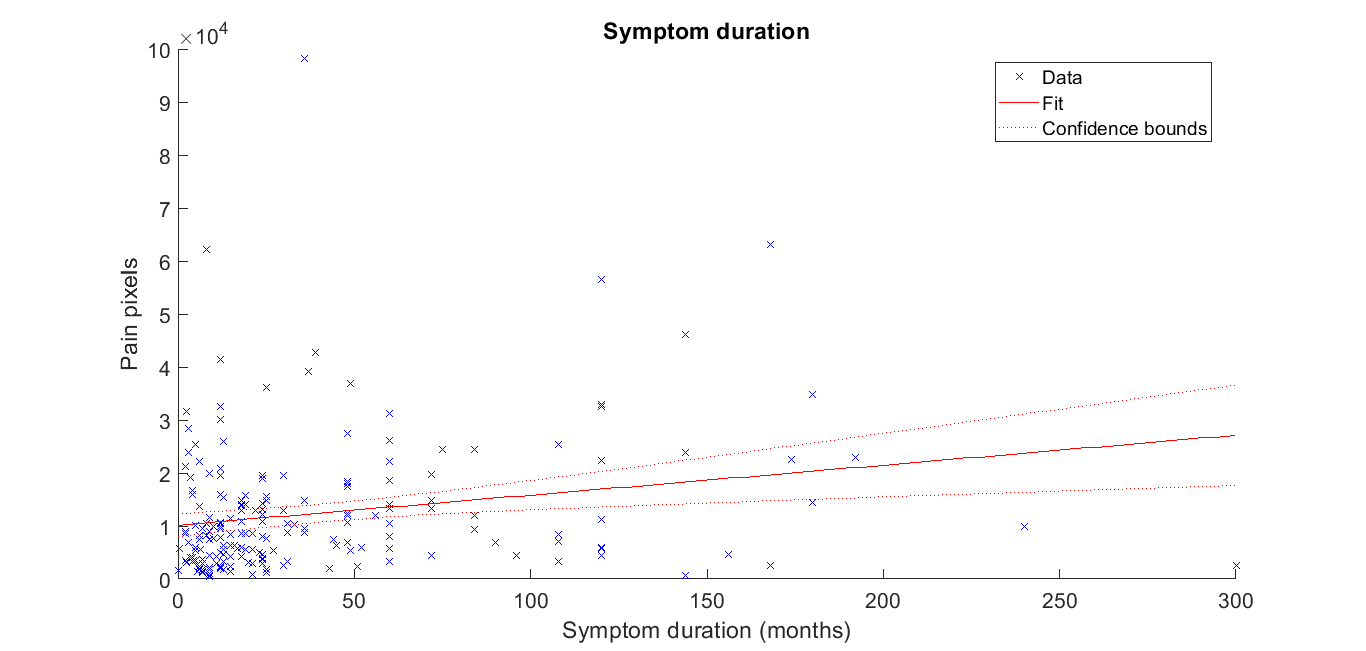
\includegraphics[width=1\textwidth]{figures/durationRegression}
\caption{A linear regression of the symptom duration and the number of pain pixels.}
\label{fig:durationRegression}
\end{figure}

\noindent
According to the figure is it assumed that there is not a correlation between the symptom duration and number of pain pixels, since there is wide spread between in the data. As a result of the linear regression model is an R-squared value on 0.046, which indicate that there is not linear correlation, because the value is close to zero.
\noindent
A linear regression model of pain intensity and the size of pain area is also made, which is illustrated in figure \ref{fig:painRegression}. \newline

\begin{figure} [H]
\centering
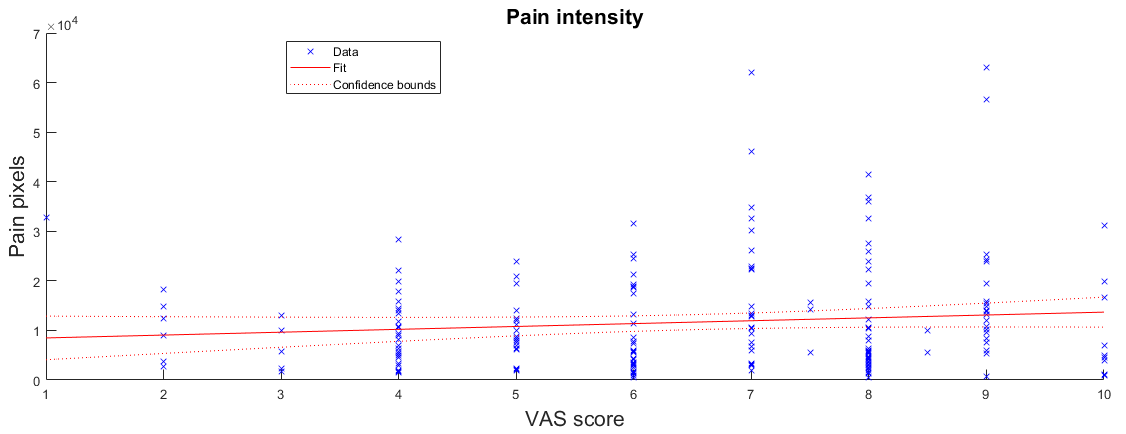
\includegraphics[width=1\textwidth]{figures/painRegression}
\caption{A linear regression fit of pain intensity stated in VAS and the size of pain area.}
\label{fig:painRegression}
\end{figure}

\noindent
Figure \ref{fig:painRegression} also indicates a wide spread in the data. The R-squared value of this model is 0.0117, which is very low, so there is no linear correlation between pain intensity and the number of pain pixels.
These linear regression models are not very suitable when trying to predict symptom duration or pain intensity from the size of pain area. However, they can be compared to the performance of the deep learning models. 
\noindent
Beside the linear regressions is the correlation between the number of active regions and either symptom duration or pain intensity investigated, which is shown in figure \ref{fig:regDuration} and figure \ref{fig:regPain}. \newline

\begin{figure} [H]
\centering
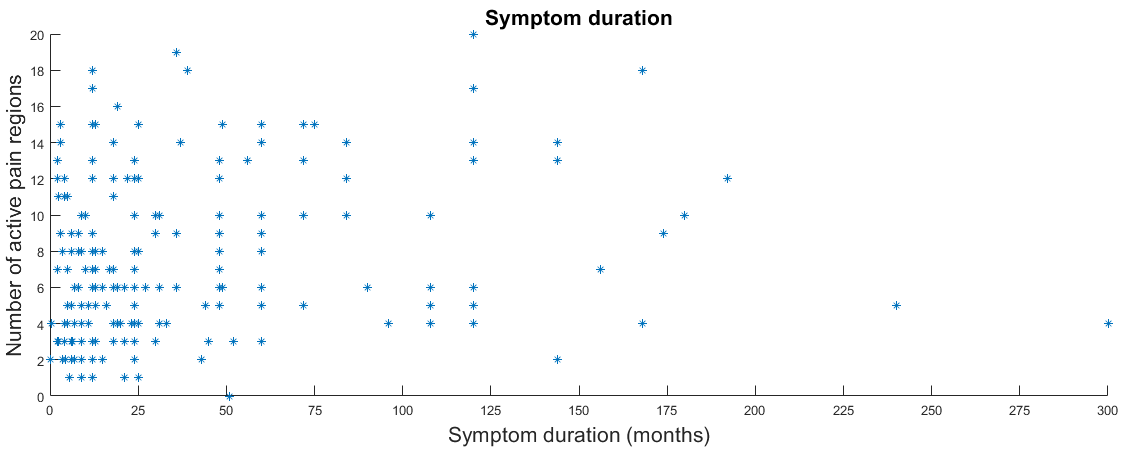
\includegraphics[width=1\textwidth]{figures/regionRegressionDuration}
\caption{Plot of the correlation between the number of active pain regions and symptom duration.}
\label{fig:regDuration}
\end{figure}

\newpage
\noindent
In figure \ref{fig:regDuration} is a dispersion of the data, which presumably means that there is not a correlation to be found between the number of regions and for how long the individuals have had PFP. 
Thereto is a figure of the correlation between the number of active pain regions and pain intensity shown in figure \ref{fig:regPain}.

\begin{figure} [H]
\centering
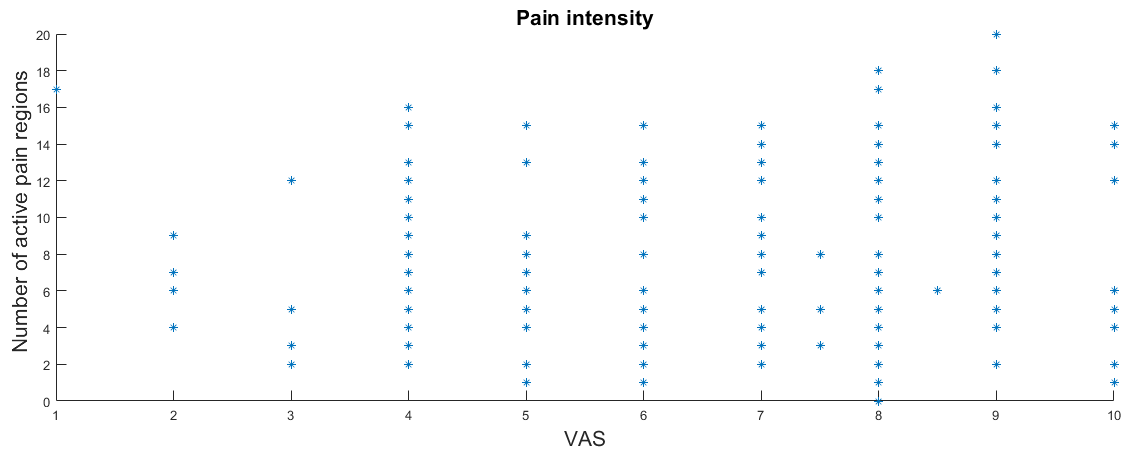
\includegraphics[width=1\textwidth]{figures/regionRegressionPain}
\caption{Plot of the correlation between the number active pain regions and pain intensity.}
\label{fig:regPain}
\end{figure}

\noindent
The figure shows once again a wide dispersion of the data. There is therefore no simple correlation between the number of active regions and pain intensity. 
\noindent
Based on the four figures is it assumed that a single feature, number of pain pixels or regions, may not have a simple correlation with the outputs, symptom duration or pain intensity. Thereto is it interesting to investigate the morphology of pain and knee regions as features in a more complicated model. 


\section{Pre-processing}
The data is pre-processed in MatLab to prepare it to the three different deep learning models. Each model has an appurtenant data representation which are prepared in three different ways. The three data representations are morphology, regions and combined, which are described in section \ref{sec:representation}. Common for the data representation is that the pain maps are imported as image-matrices whereafter the matrices are resized, since the given data was collected at different resolutions (screen sizes). Furthermore, the matrices are cropped to sort out unnecessary data like the areas inferior and superior to the knee.
Before the data is used as an input in the deep learning models each matrix, which represent an image, is converted into a vector whereafter they are assembled in one matrix for each data representation. To get additional information associated with the pain maps, is gender added by including a column vector to the three matrices.
In addition to the input, the deep learning models need an output to train the models. The output, which is either symptom duration or pain intensity, is likewise added as a column vector.
The following sections describe the pre-processing of the individual data representations.

\subsection{Morphology-representation} \label{sec:Morph}
The first representation of data is a binary matrix of the original pain maps.
Firstly, the image of the original pain map is gray-scaled to get a one-dimensional matrix instead of a three-dimensional RGB-matrix. This matrix is then converted into a matrix consisting of zeroes and ones, where the pain pixels are symbolized with ones. An original pain map and a pain map consisting of a binary matrix is shown in figure \ref{fig:cropbin7}.

\begin{figure} [H]
\centering
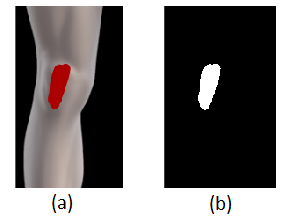
\includegraphics[width=0.7\textwidth]{figures/cropbin7}
\caption{(a) Original pain map and (b) image consisting of a binary matrix where white color represents the pain pixels.}
\label{fig:cropbin7}
\end{figure}

\noindent
An illustration of this data representation is created to convey how the data is assembled and transferred to the model. The illustration is shown in figure \ref{fig:binmatrix}, where a matrix containing image-vectors for all the pain maps and appurtenant gender and either symptom duration or pain intensity.

\begin{figure} [H]
\centering
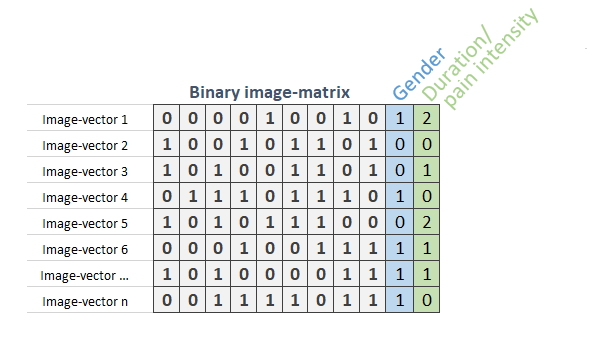
\includegraphics[width=0.8\textwidth]{figures/binaryimagematrix}
\caption{An illustration of the matrix of the morphology-representation. The matrix consist of image-vectors for each individuals where the two last columns indicate the appurtenant gender (blue column vector) and either symptom duration or pain intensity (green column vector). The image-vectors have a length equal to the number of pixels in the pain maps.}
\label{fig:binmatrix}
\end{figure}


\subsection{Regions-representation}
The second representation of the data is a matrix consisting of vectors with 20 values which indicate pain in relation to the knee regions.
An image of the knee regions as shown in figure \ref{fig:atlas} are converted into a matrix consisting of 20 values, which represent each knee regions. This matrix is superimposed to the binary image of the pain map, which results in a matrix with pain pixels represented in each knee region. In figure \ref{fig:binregions} are the knee regions and the pain associated with the regions illustrated.

\begin{figure} [H]
\centering
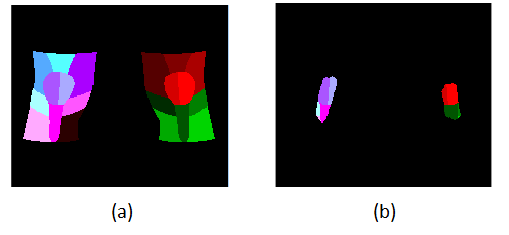
\includegraphics[width=0.8\textwidth]{figures/binregions}
\caption{(a) Knee regions and (b) pain in the specific regions.}
\label{fig:binregions}
\end{figure}

\noindent
After superimposing the two matrices, knee regions and pain pixels, the number of pixels in each active knee region is found. This number is compared to the total number of pixels that are in each knee region, so knee regions with less than 5 percent pain are excluded. The threshold on 5 percent is chosen based on the analysis in section \ref{sec:Selectthreshold}. As a result a vector with 20 values is created with zeros and ones, where one represent an active region. This data representation is implemented in the deep learning models the same way as the morphology-representation, which is illustrated in figure \ref{fig:binmatrix}. The only difference is that the length of the image-vectors respond to the 20 regions, and therefore are there only 20 values in this data representation.


\subsection{Combined-representation}
The third representation of the data is a matrix consisting of individuals’ pain divided into the knee regions.
\noindent
In this representation the superimposed matrix from the region-representation is used. Since the data representation should reflect the morphology of the pain and divide the pain into the different knee regions is one-hot encoding used. One-hot encoding is a way to separate categorical data into binary data \citep{Harris2012}. This means that the 20 values for each knee region do not have a correlation. After one-hot encoding, the superimposed matrix consists of 20 layers where each layer represents a knee region. An illustration of this data representation is shown in figure \ref{fig:onehot}.


\begin{figure} [H]
\centering
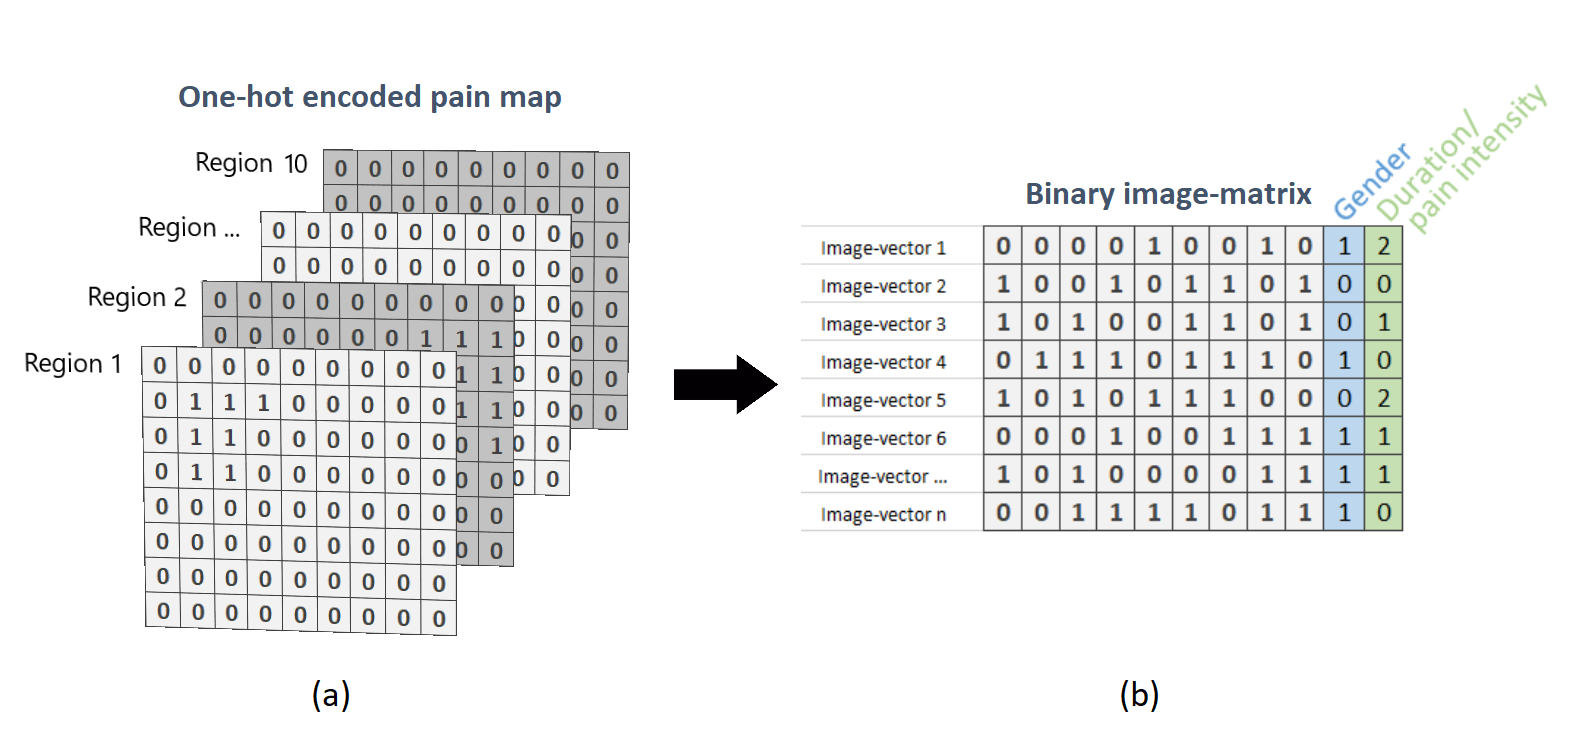
\includegraphics[width=1\textwidth]{figures/onehotmatrix}
\caption{(a) An illustration of the one-hot encoded pain map and (b) shows the images-vectors in one assembled matrix with gender and either symptom duration or pain intensity.}
\label{fig:onehot}
\end{figure}
